\documentclass[10pt,a4paper]{article}
\usepackage[utf8]{inputenc}
\usepackage[german]{babel}
\usepackage[T1]{fontenc}
\usepackage{amsmath}
\usepackage{amsfonts}
\usepackage{amssymb}
\usepackage{url}
\usepackage{graphicx}
\usepackage{draftwatermark}
\usepackage{raleway}
\setmainfont{Raleway}


\author{Ben Oswald}
\title{Was ist Freifunk?}

\usepackage{graphicx}
\usepackage{draftwatermark}
\SetWatermarkText{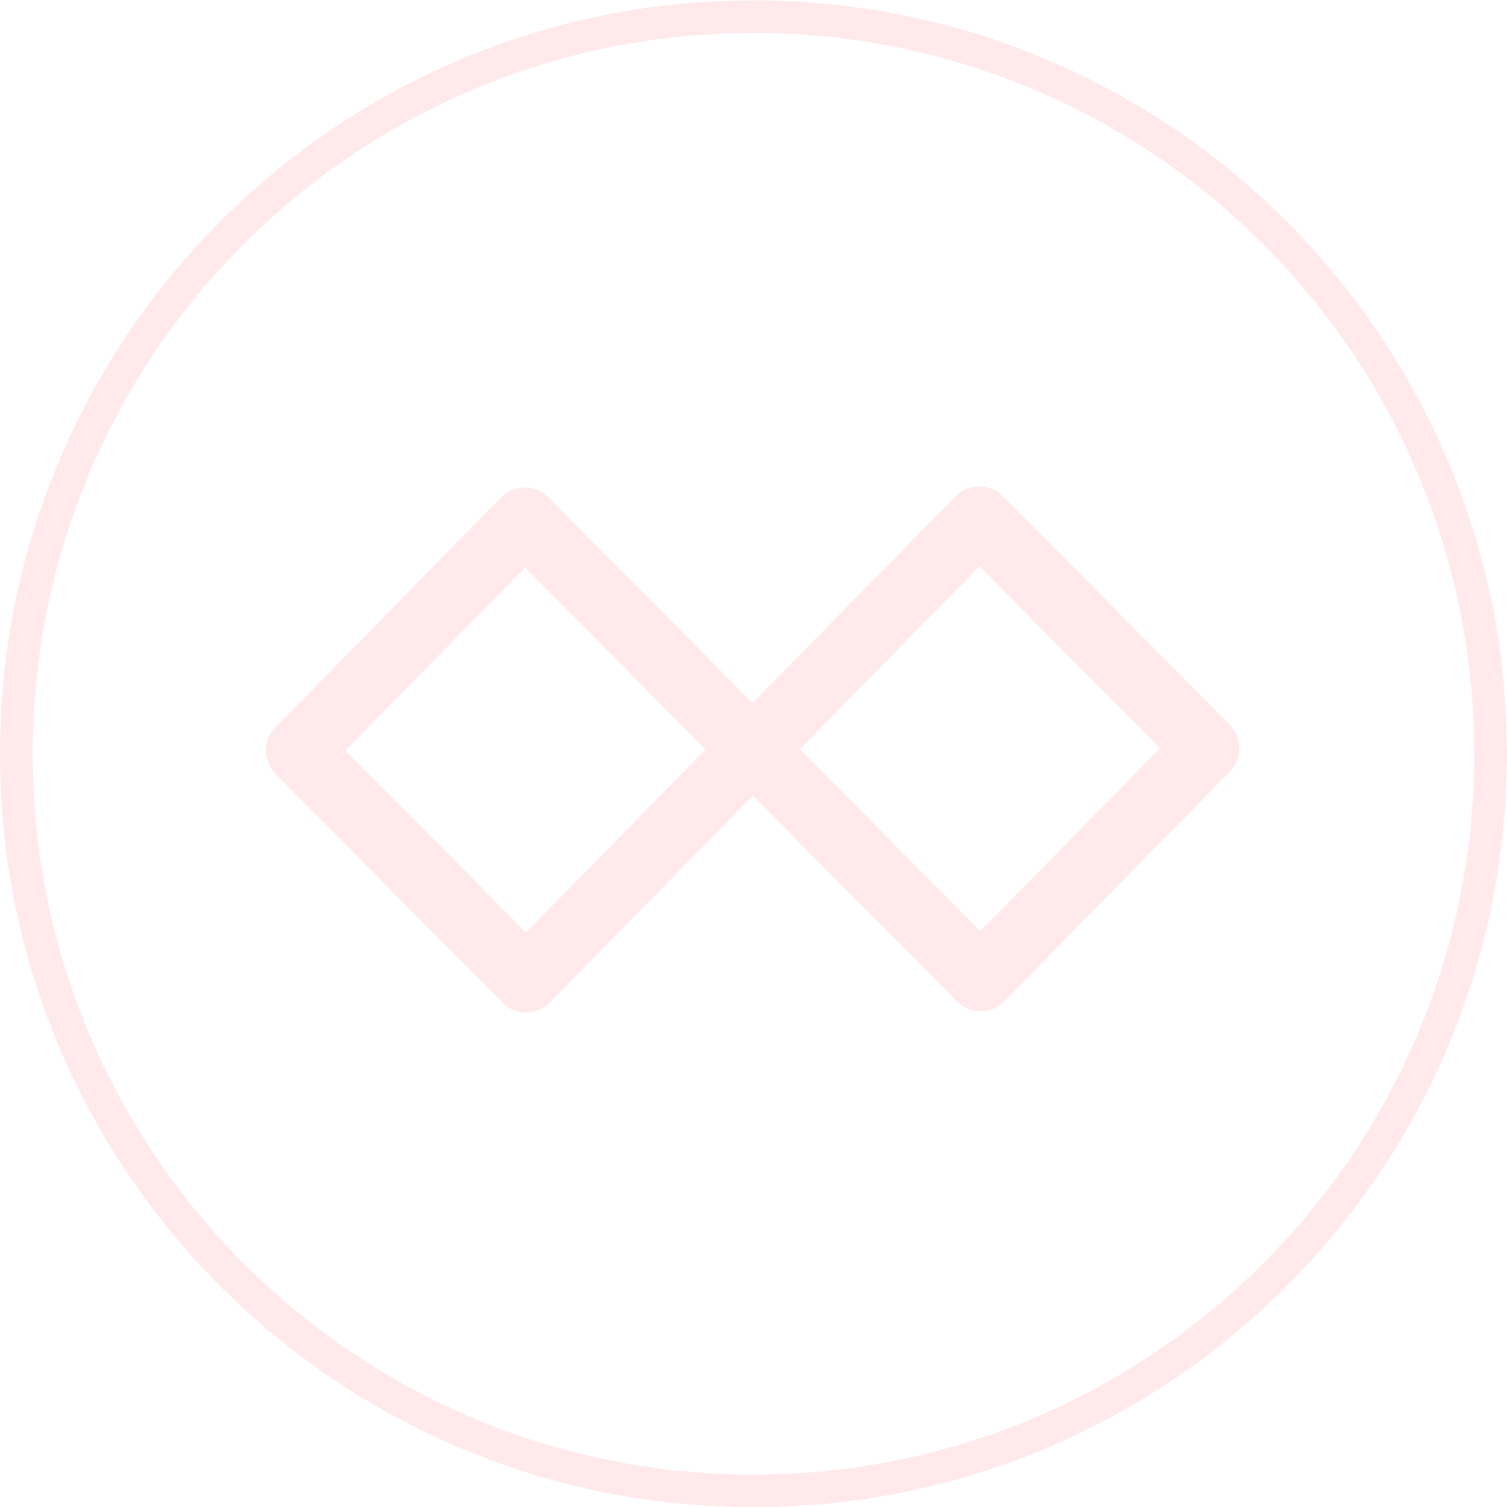
\includegraphics[angle=-45, scale=12]{ffrn_watermark.png}}

\begin{document}
\pagenumbering{gobble}

\section*{Was ist Freifunk?}

Freifunk ist die Idee eines freien, unzensierten, unlimitierten und dezentralen WLAN Netzwerks, betrieben
durch die Nutzer selbst.
\\\\
Netzwerke, insbesondere das Internet, sind heute wichtiger denn je und quasi jeder nutzt sie mehrmals
täglich. Doch häufig gibt es keinen wirklich freien Zugang zum Netz. Entweder wir müssen uns mit dem geringen
Volumen eines Mobilfunkanbieters rumärgern oder es gibt zwar einen WLAN Hotspot, denn wir für 30 Minuten kostenlos
Nutzen können, dafür müssen wir uns aber erst kompliziert registrieren und bei längerer Nutzung fallen Kosten an.
Das wollen wir ändern, auch weil wir damit im europäischen Vergleich auf einem der hintersten Ränge liegen.
\\\\
Wir ermöglichen, fern jedem kommerziellen Interesse, den Menschen in unserer Region einen freien Zugang zum Netz. Außerdem
geben wir den Nutzern einen Teil der Kontrolle über das Netz zurück, das diese täglich nutzen. Eine gewisse Unabhängigkeit
von den großen Telekommunikationsanbietern also. Dazu baut Freifunk ein selbst verwaltetes WLAN-Netz im Rhein Neckar Gebiet.
Dieses formt sich heute schon aus Hunderten von WLAN Accespoints, die von Freifunkern in privaten Wohnungen, Geschäften 
und in der Gastronomie betrieben werden. Eine Übersicht wo es schon überall Freifunk gibt, findet sich auf unserer Karte\footnote{http://map.ffrn.de/}.
\\\\
Um Teil des Freifunk Rhein Neckar Netzes zu werden, muss ein Router mit unserer Software bespielt werden, das sogenannte \glqq flashen\grqq.
Anschließend kann der neue Freifunk Knoten, so nennen wir die Router mit unserer Software, mit dem eigenen Internetanschluss verbunden werden,
um einen Teil der Bandbreite den Menschen in der Umgebung zur Verfügung zu stellen.\\
Sollten ein Knoten keinen eigenen Zugang zum Internet haben (Mesh only), es gibt aber einen Knoten mit Internet in der Nähe, können sich diese Knoten über
das Mesh miteinander verbinden. Dadurch können Nutzer das Netz auch über den Knoten nutzen, der selber gar keinen Internetzugang hat. Dies funktioniert,
da der \glqq Mesh Only\grqq-Router seine Daten an den Knoten mit eigenem Internetzugang weiterleitet.
\\\\
Um den Betreiber eines Knotens vor der in Deutschland gefürchteten Störerhaftung zu schützen, werden alle Daten, die im Freifunk WLAN erzeugt werden, über spezielle
Server geleitet. Diese Server bzw. Gateways werden durch den Freifunk Rhein-Neckar e.V. betrieben und leiten die Daten ins Internet weiter. Durch diese
VPN\footnote{\textbf{V}irtual \textbf{P}rivate \textbf{N}etwork} Gateway Technik, steht als Absender auf den Daten der Name des Vereins. Dieser wiederum ist durch die gesetzlichen Regelungen als ISP\footnote{\textbf{I}nternet \textbf{S}ervice \textbf{P}rovider} tätig und daher nicht als Störer
haftbar. Da wir laut Datenschutzgesetz weder Daten über unsere Nutzer erheben dürfen, noch dies überhaupt wollen, könnten wir bei einer Abmahnung keine Informationen weitergeben.
So sind alle Beteiligten vor rechtlichen Risiken geschützt.
\newpage
\noindent
Neben der Vermittlung von Wissen über den Aufbau und die Funktionsweise von freien Datennetzen, hat es sich Freifunk Rhein-Neckar mit dem Projekt \glqq FFRN Hilft\grqq{} zum Ziel gesetzt, auch Flüchtlingen und
sozial benachteiligten Menschen den Zugang zum Internet zu ermöglichen. Denn häufig ist das Internet für die Flüchtlinge die einzige Möglichkeit mit Verwandten und Bekannten in der Heimat in
Kontakt zu kommen. Daher befindet sich Freifunk Rhein Neckar mit verschiedenen Organisationen zur Flüchtlingshilfe im Gespräch, um einen Weg zu finden, wie wir diesen Menschen gemeinsam helfen können.
\\\\
Da wir ein solch ehrgeiziges und großes Projekt nicht ohne eine engagierte, ehrenamtliche Community stemmen können, suchen wir immer nach Unterstützerinnen und Unterstützern. Wenn Du die Idee hinter Freifunk also
unterstützen möchtest, mach mit! Alle dazu nötigen Informationen findest du auf unserer Website https://freifunk-rhein-neckar.de und bei Fragen erreichst du uns per Mail unter info@freifunk-rhein-neckar.de
\\\\
Eine sehr schöne Zusammenfassung was Freifunk ist, findet sich auch nochmal hier als Video: \url{https://vimeo.com/64814620}

\end{document}